\section{Deep Learning Techniques}
%%%%%%%%%%%%%%%%%%%%%%%%%%%%%%%%%%%%%%%%%%%%%%%%%%%%%%%%%%%%%%%%%%%%%%%%
\begin{frame}{Multi-Layer Perceptron}
    \begin{figure}[t]
        \centering
        \resizebox{.6\linewidth}{!}{\input{tikz/MLP}}
        \caption{Multi-Layered Perceptron (adapted from \textcite{neutelings2021_nn})}
        % ]{A simple MLP with an input dimension of 4 (green nodes), three hidden layers (blue nodes), and an output dimension of 3 (red nodes). Each node is connected to every node in the previous and next layer. The lines represent the weights, and each  node has an associated bias. Figure adapted from 
        \label{fig:MLP}
    \end{figure}
\end{frame}

\begin{frame}{CNN Architecture}
    \begin{figure}[t]
        \centering 
        \resizebox{.6\linewidth}{!}{\begin{tikzpicture}[
    2d-arr/.style={matrix of nodes, row sep=-\pgflinewidth, column sep=-\pgflinewidth, nodes={draw}}
  ]

  \matrix (mtr) [2d-arr] {
  |[fill=red!30]| 0  & |[fill=red!30]| 0  & |[fill=red!30]| 0  & |[fill=red!30]| 0  & |[fill=red!30]| 0  & |[fill=red!30]| 0 \\
  |[fill=red!30]| 0  & |[fill=orange!30]| 1 & |[fill=orange!30]| 1 & |[fill=orange!30]| 1 &  0 & |[fill=red!30]| 0 \\
  |[fill=red!30]| 0  & |[fill=orange!30]| 0 & |[fill=orange!30]| 1 & |[fill=orange!30]| 1 &  1 & |[fill=red!30]| 0 \\
  |[fill=red!30]| 0  & |[fill=orange!30]| 0 & |[fill=orange!30]| 1 & |[fill=orange!30]| 1 & 0 & |[fill=red!30]| 0 \\
  |[fill=red!30]| 0  & 1 & 1 & 0 & 0 & |[fill=red!30]| 0 \\
  |[fill=red!30]| 0  & |[fill=red!30]| 0  & |[fill=red!30]| 0  & |[fill=red!30]| 0  & |[fill=red!30]| 0  & |[fill=red!30]| 0 \\
  };

  \node[below=of mtr-5-4] {$4\times4$ input with padding};

  \node[right=0.2em of mtr] (str) {$*$};

  \matrix (K) [2d-arr, right=0.2em of str, nodes={draw, fill=teal!30}] {
    1 & 0 &1\\
    0 & 1 &0\\
    1 & 0 & 1\\
  };
  \node[below=of K-2-2] {$3\times3$ filter};

  \node[right=0.2em of K] (eq) {$=$};

  \matrix (ret) [2d-arr, right=0.2em of eq] {
  2 & 2 & 3 &  1\\
  2 & |[fill=blue!80!black!30]| 4 & 3 & 3\\
  2 & 3 & |[fill=orange!30]| 4 & |[fill=orange!30]| 1 \\
  2 & 2 & |[fill=orange!30]| 1 & |[fill=orange!30]| 1 \\
  };
  \node[below=of ret-4-3] {$4\times4$ tensor};

  \node[right=0.2em of ret] (ra) {$\xrightarrow[]{\text{Max Pooling}}$};

\matrix (pool) [2d-arr, right=0.2em of ra] {
  4 & 3 \\
  3 & |[fill=blue!80!black!30]| 4 \\
  };
  \node[below=of pool-2-2] {$2\times2$ tensor};

  \draw[dashed, teal] (mtr-2-4.north east) -- (K-1-1.north west);
  \draw[dashed, teal] (mtr-4-4.south east) -- (K-3-1.south west);

  \draw[dashed, blue!80!green] (K-1-3.north east) -- (ret-2-2.north west);
  \draw[dashed, blue!80!black] (K-3-3.south east) -- (ret-2-2.south west);

  \draw[dashed, blue!80!green] (K-1-3.north east) -- (ret-2-2.north west);
  \draw[dashed, blue!80!black] (K-3-3.south east) -- (ret-2-2.south west);

\draw[dashed, blue!80!green] (ret-3-4.north east) -- (pool-2-2.north west);
  \draw[dashed, blue!80!black] (ret-4-4.south east) -- (pool-2-2.south west);

\end{tikzpicture}
}
        \caption{CNN Unit ( adapted from \textcite{neutelings2022_conv})}
        \label{fig:convolution}
    % \end{figure}
    % \begin{figure}[t]
    %     \centering
        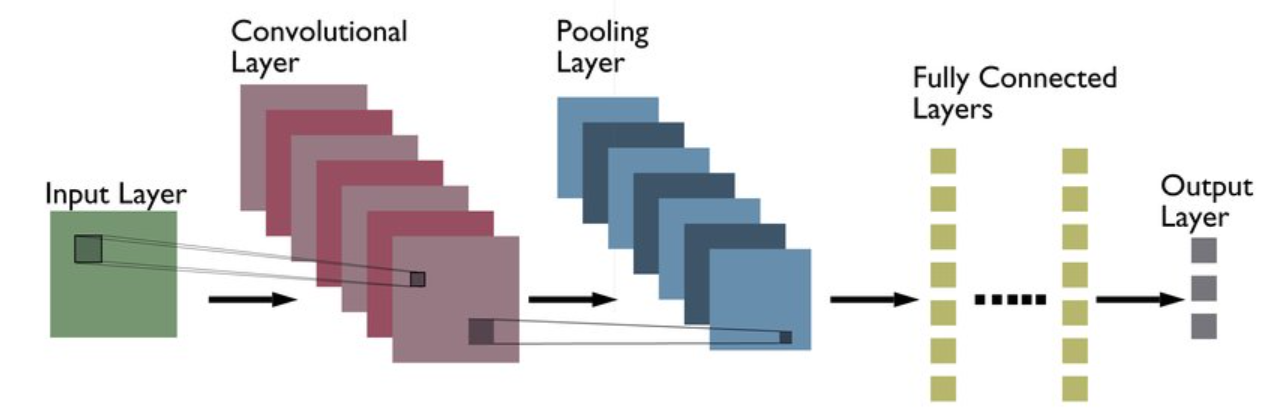
\includegraphics[width=.8\linewidth]{figures/Typical-CNN-architecture.png}
        \caption{Traditional CNN Architecture for Classification (adapted from \cite{kumar2022_cnn})}
        \label{fig:CNN}
    \end{figure}
\end{frame}

\begin{frame}{2D CNN Performance}
    \begin{figure}
        \centering
        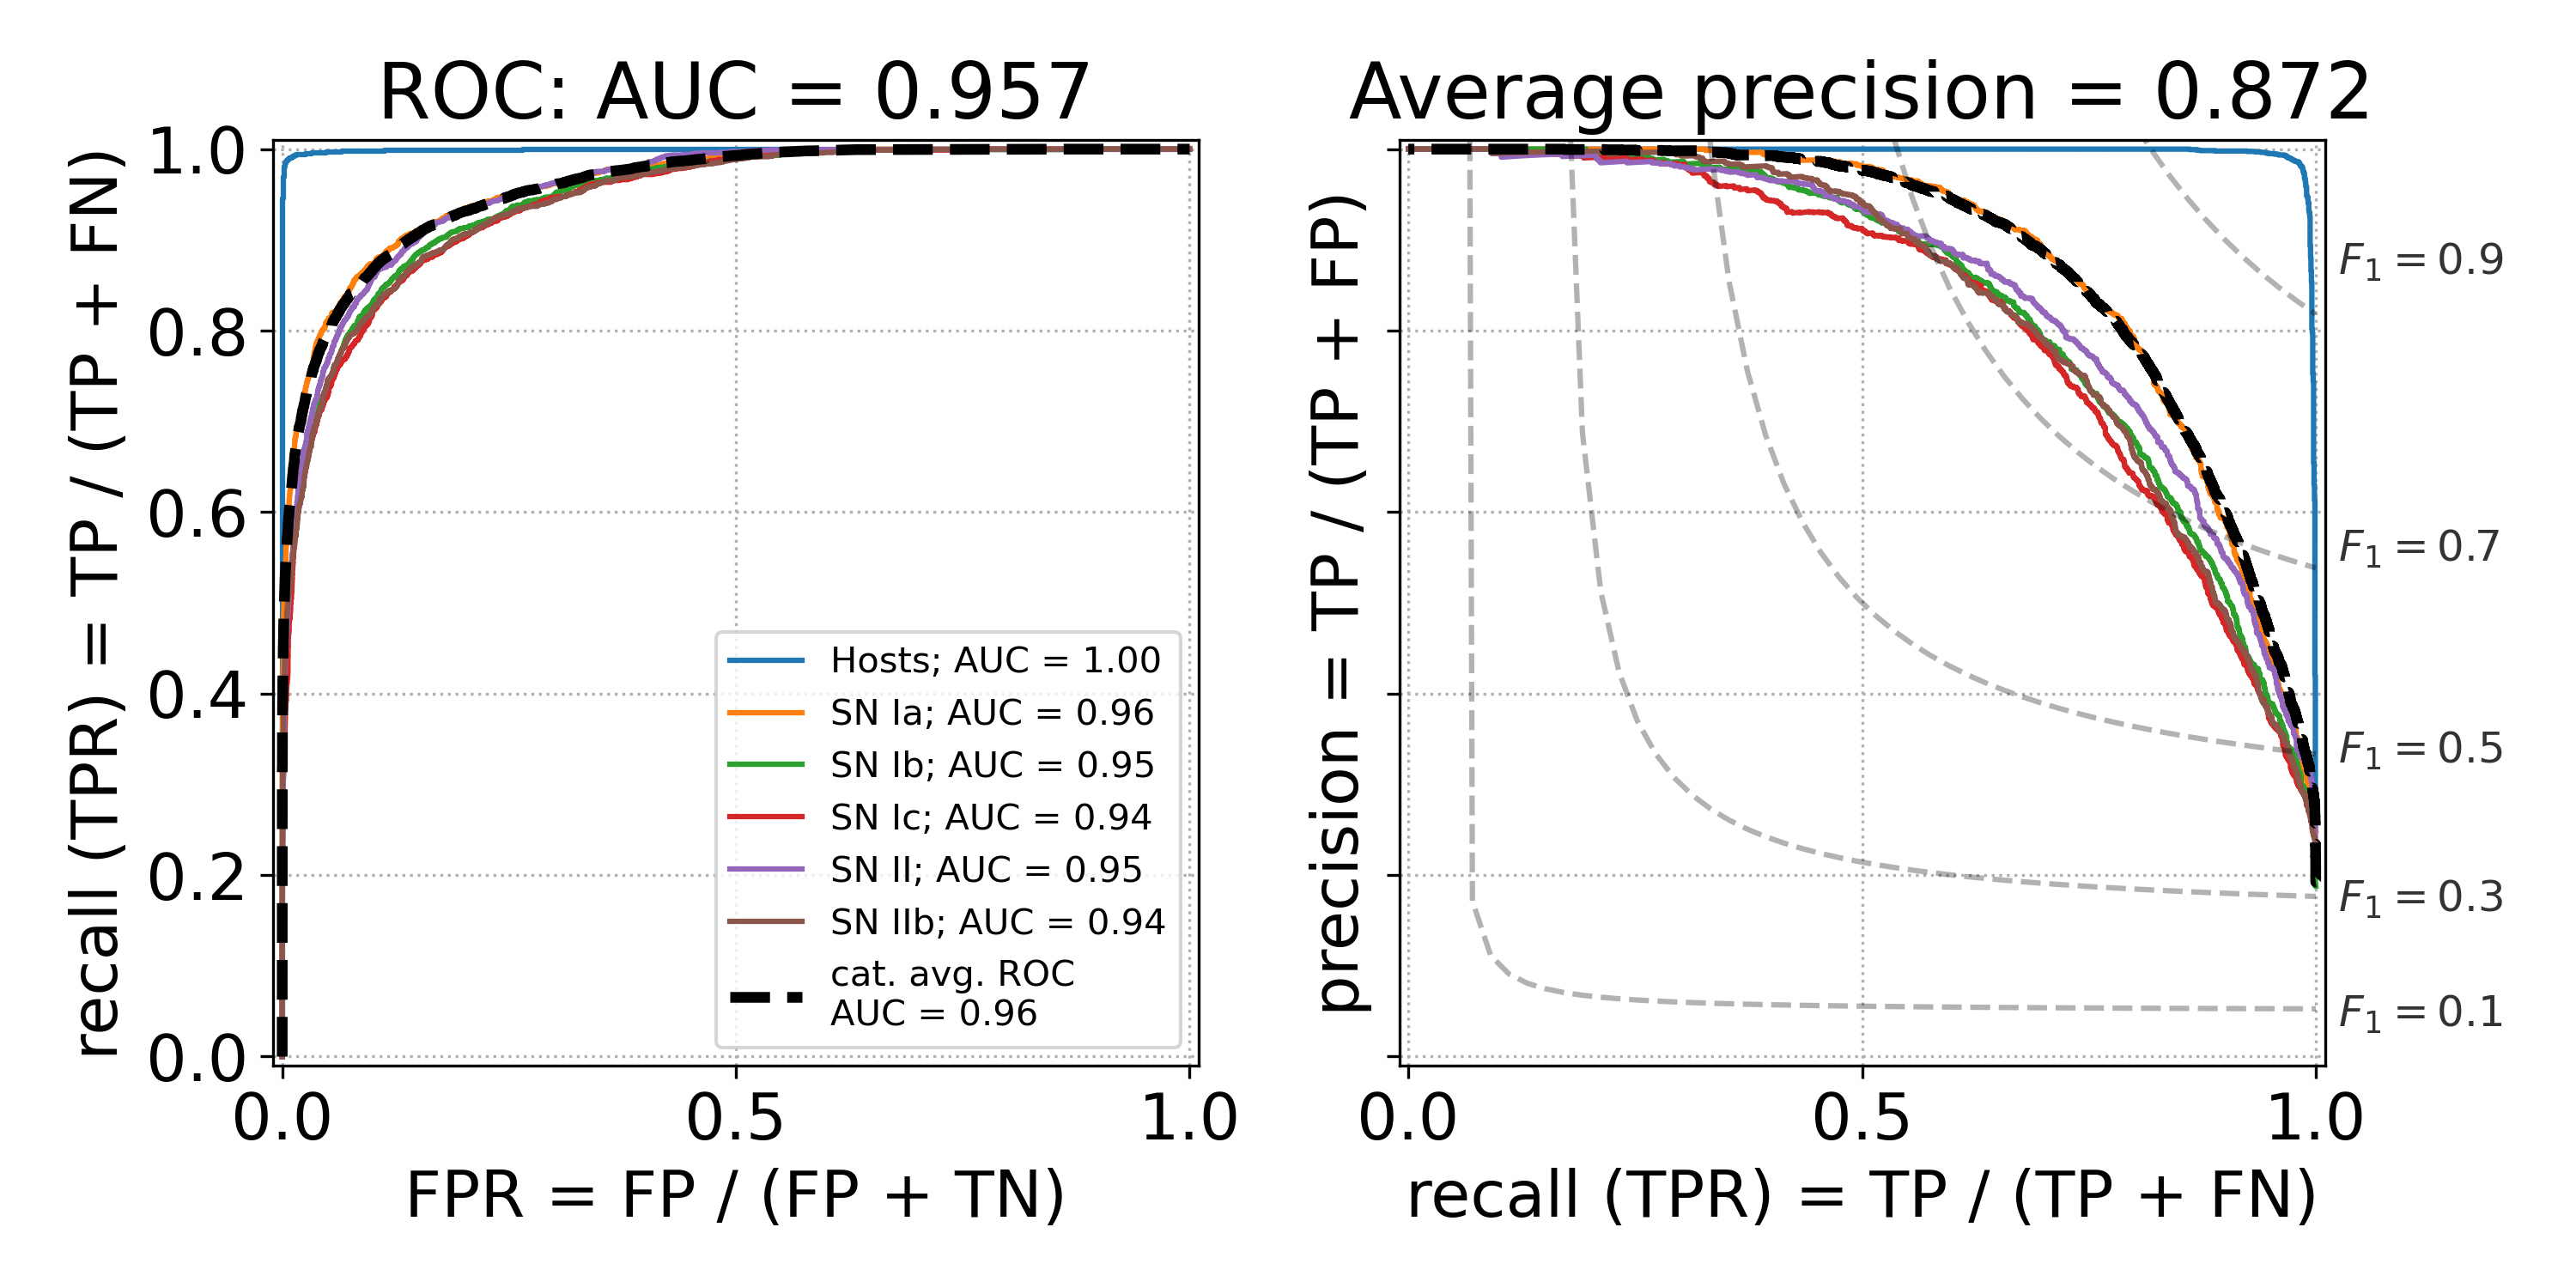
\includegraphics[height=2.8cm]{figures/cnn/cnn_rocfull.png}
        \quad
        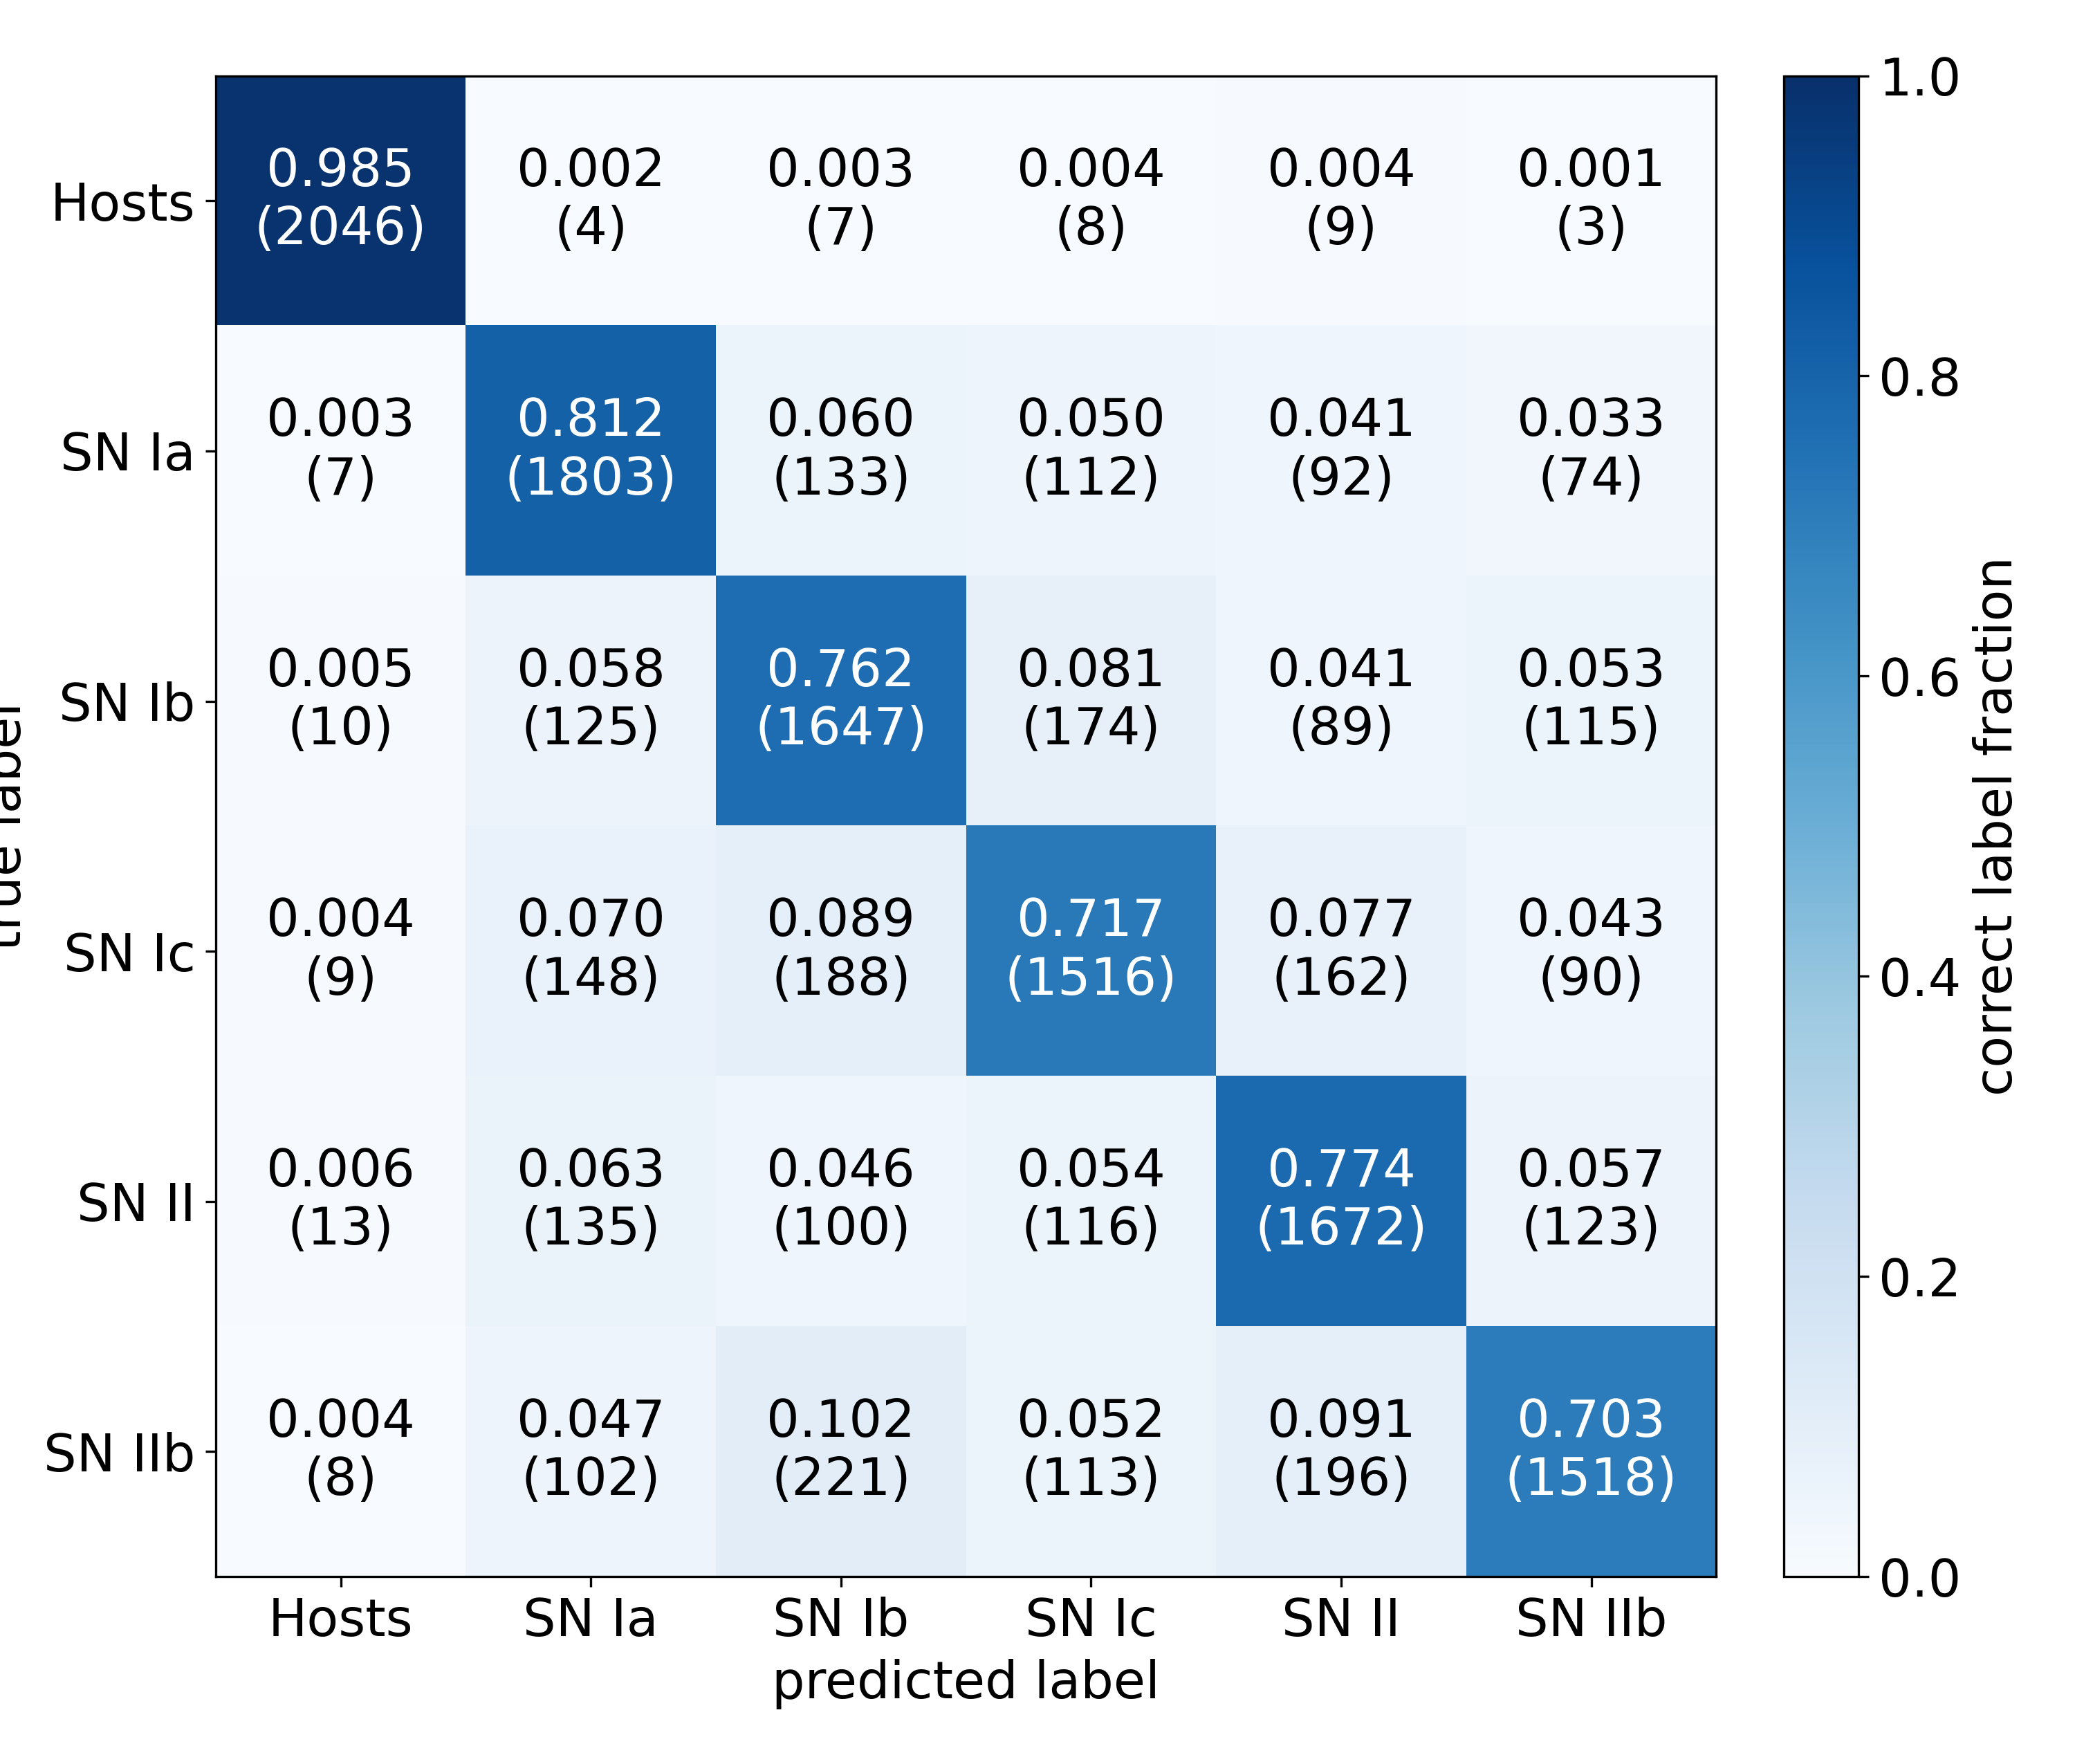
\includegraphics[height=2.8cm]{figures/cnn/cnn_cmfull.png}
        \caption{CNN Classifier}
%     \end{figure}
% \end{frame}

% \begin{frame}
%     \begin{figure}[t!]
%         \centering
        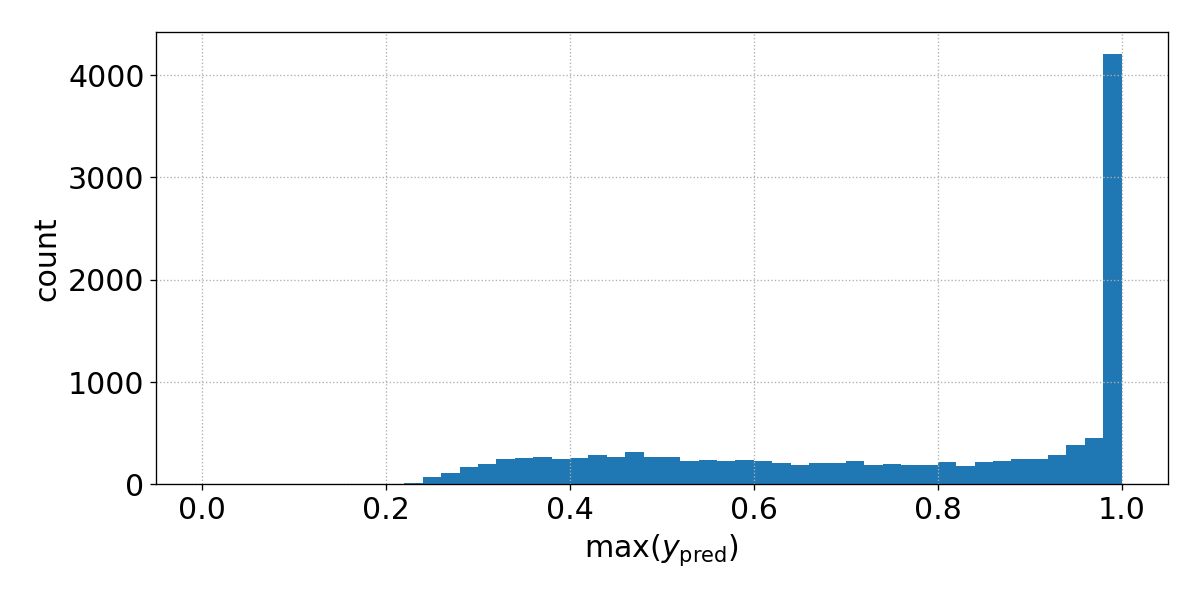
\includegraphics[width=0.5\textwidth]{figures/cnn/cnn_max_ypred.png}
        \caption{CNN's Maximum Output Vector\label{fig:cnn_max}}
    \end{figure}
\end{frame}

\begin{frame}{CNN Cut to Increase Performance}
    \begin{figure}[b]
        \centering
        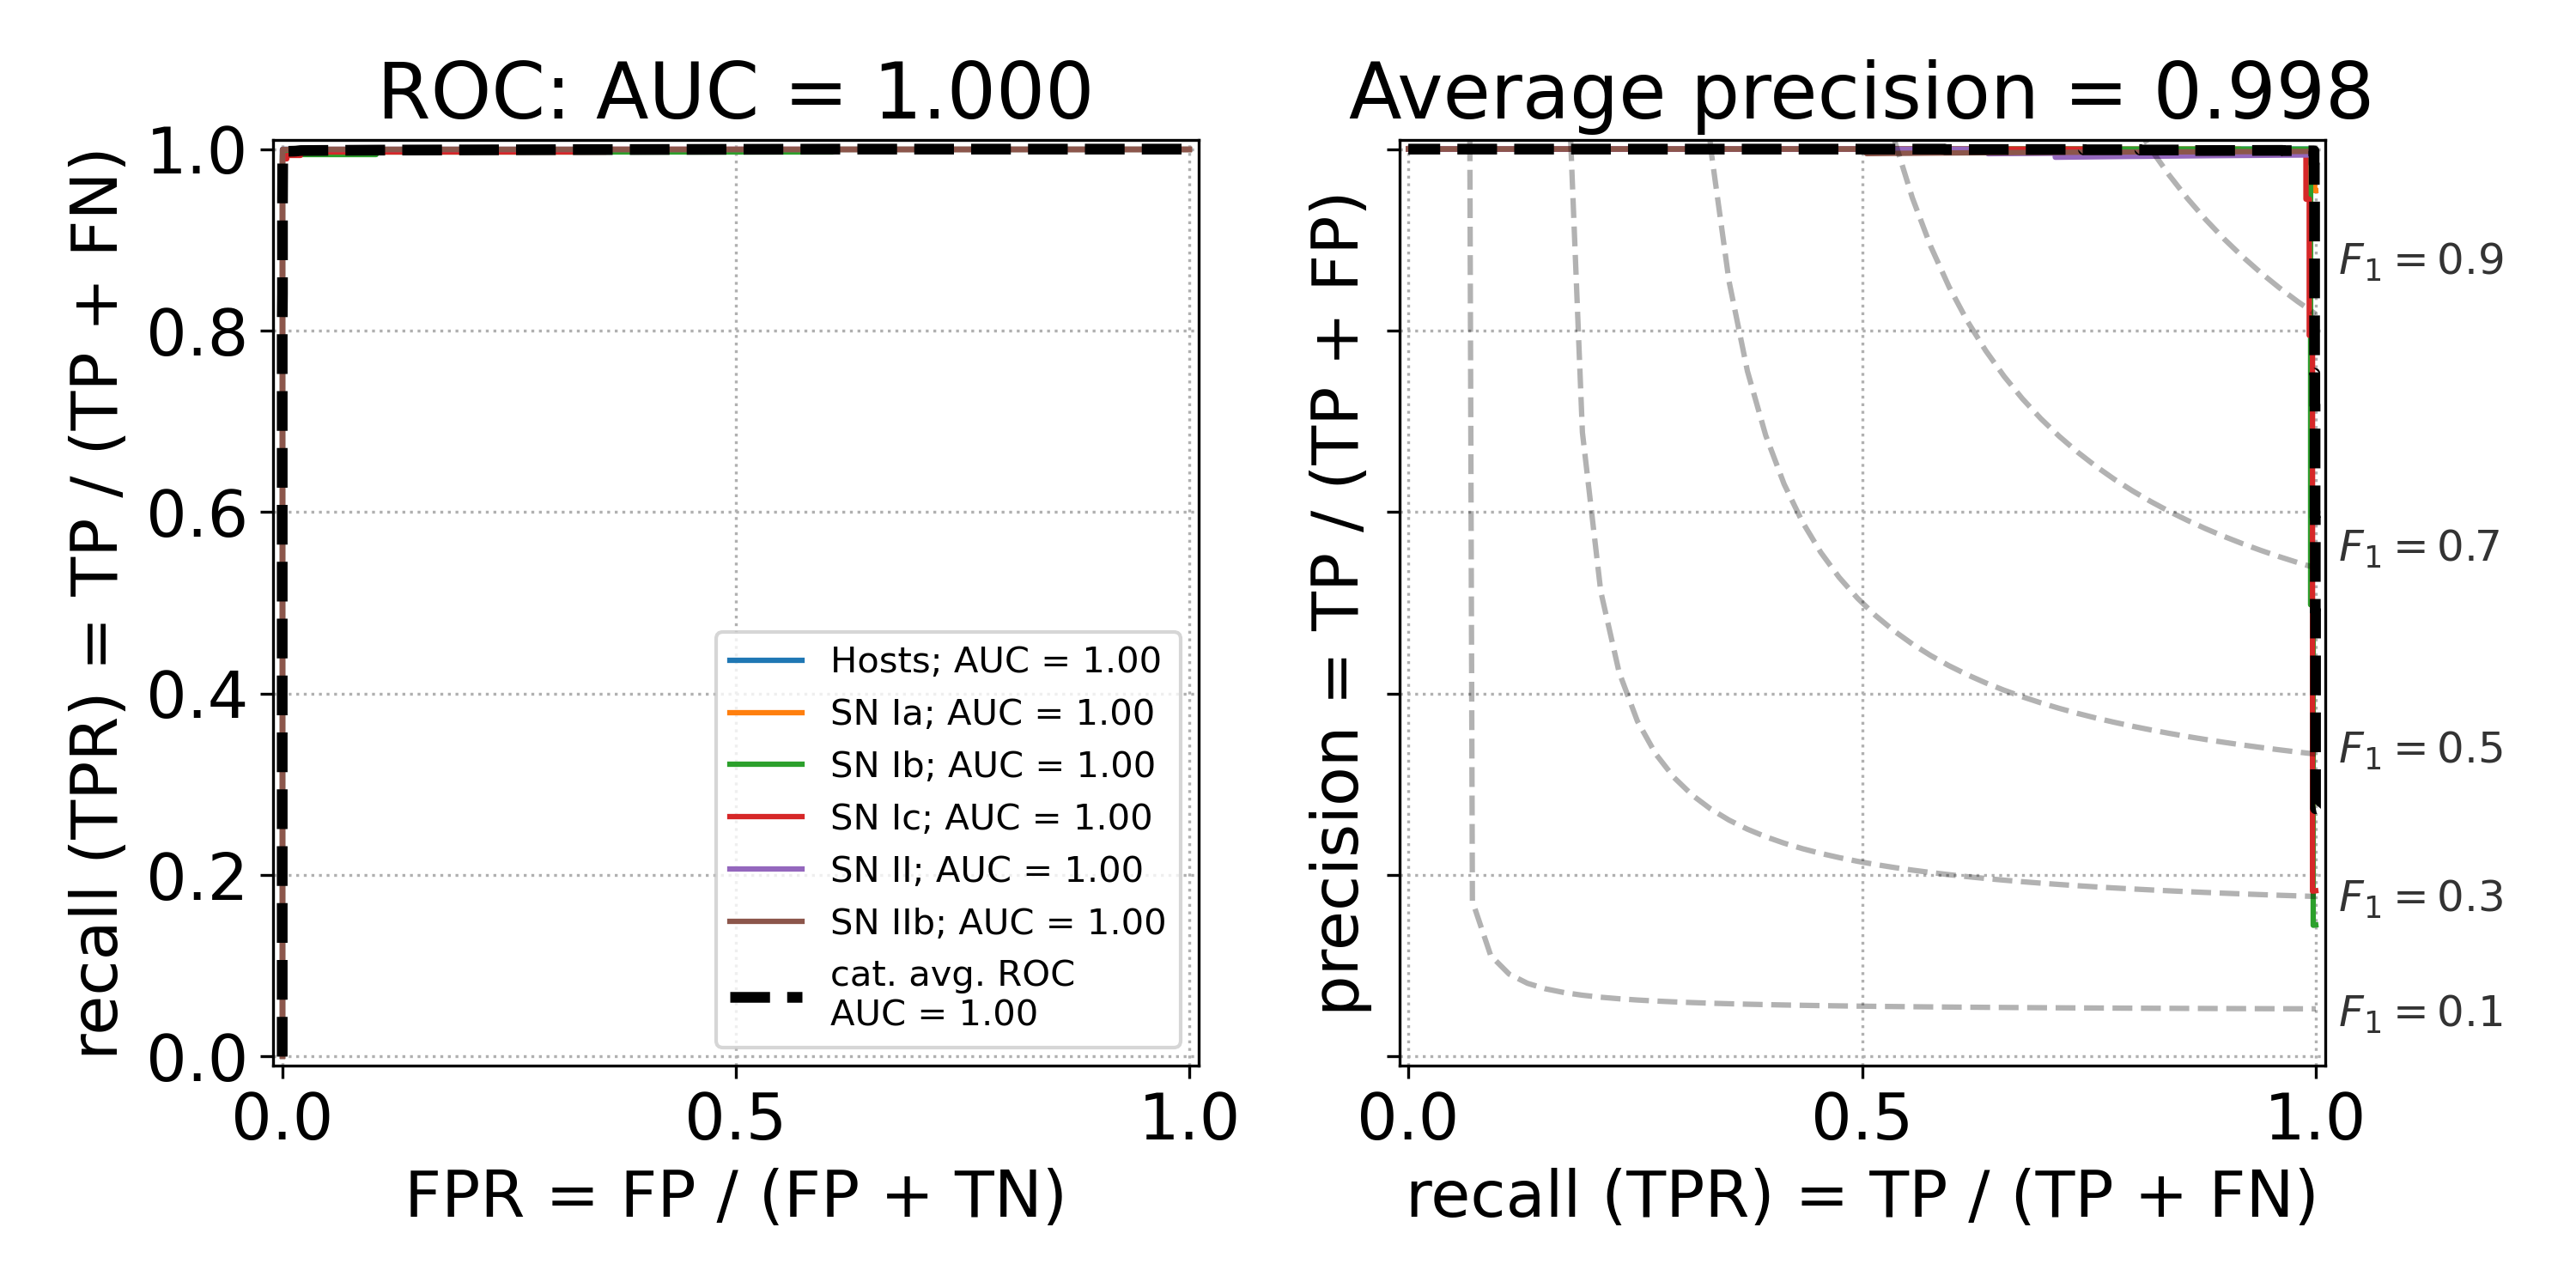
\includegraphics[height=2.6cm]{figures/cnn/cnn_roc99.png}
        \quad
        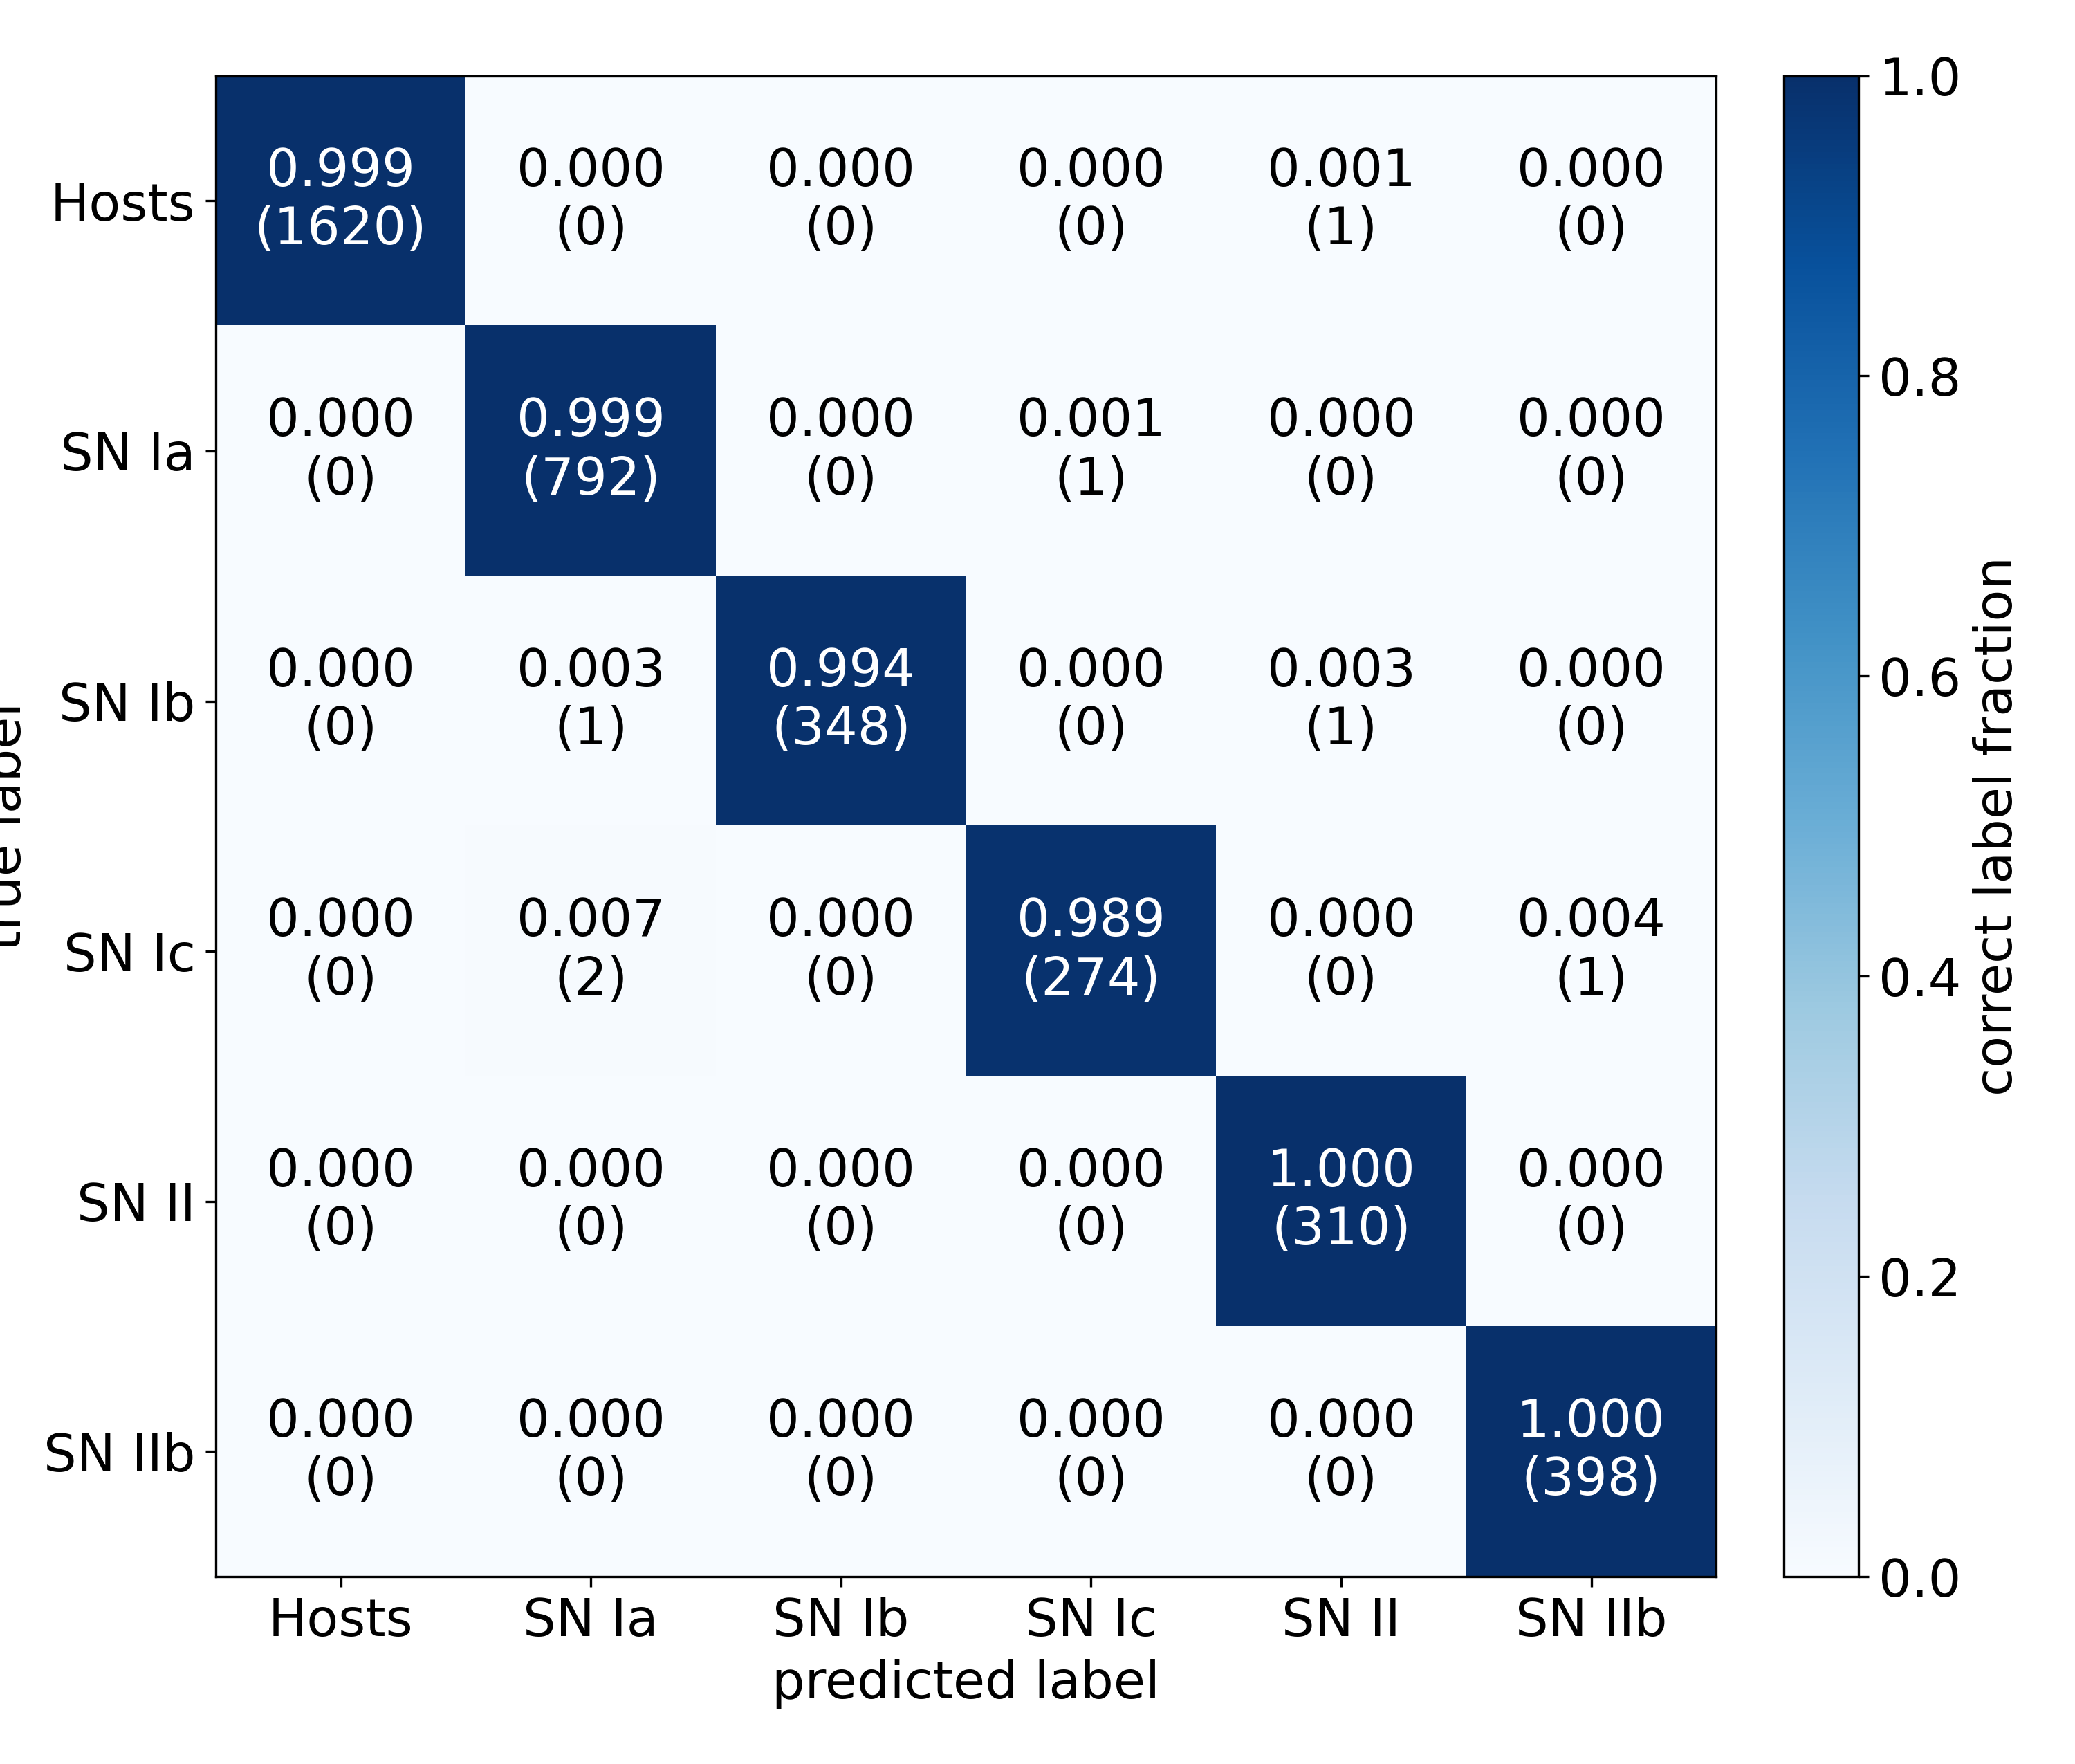
\includegraphics[height=2.6cm]{figures/cnn/cnn_cm99.png}
        \caption{CNN Classifier 99\% confidence cut (28.8\% remaining)}
    \end{figure}
\end{frame}


\begin{frame}{The Transformer Architecture}
\begin{columns}
\column{.4\textwidth}
    \begin{figure}[ht]
        \centering
        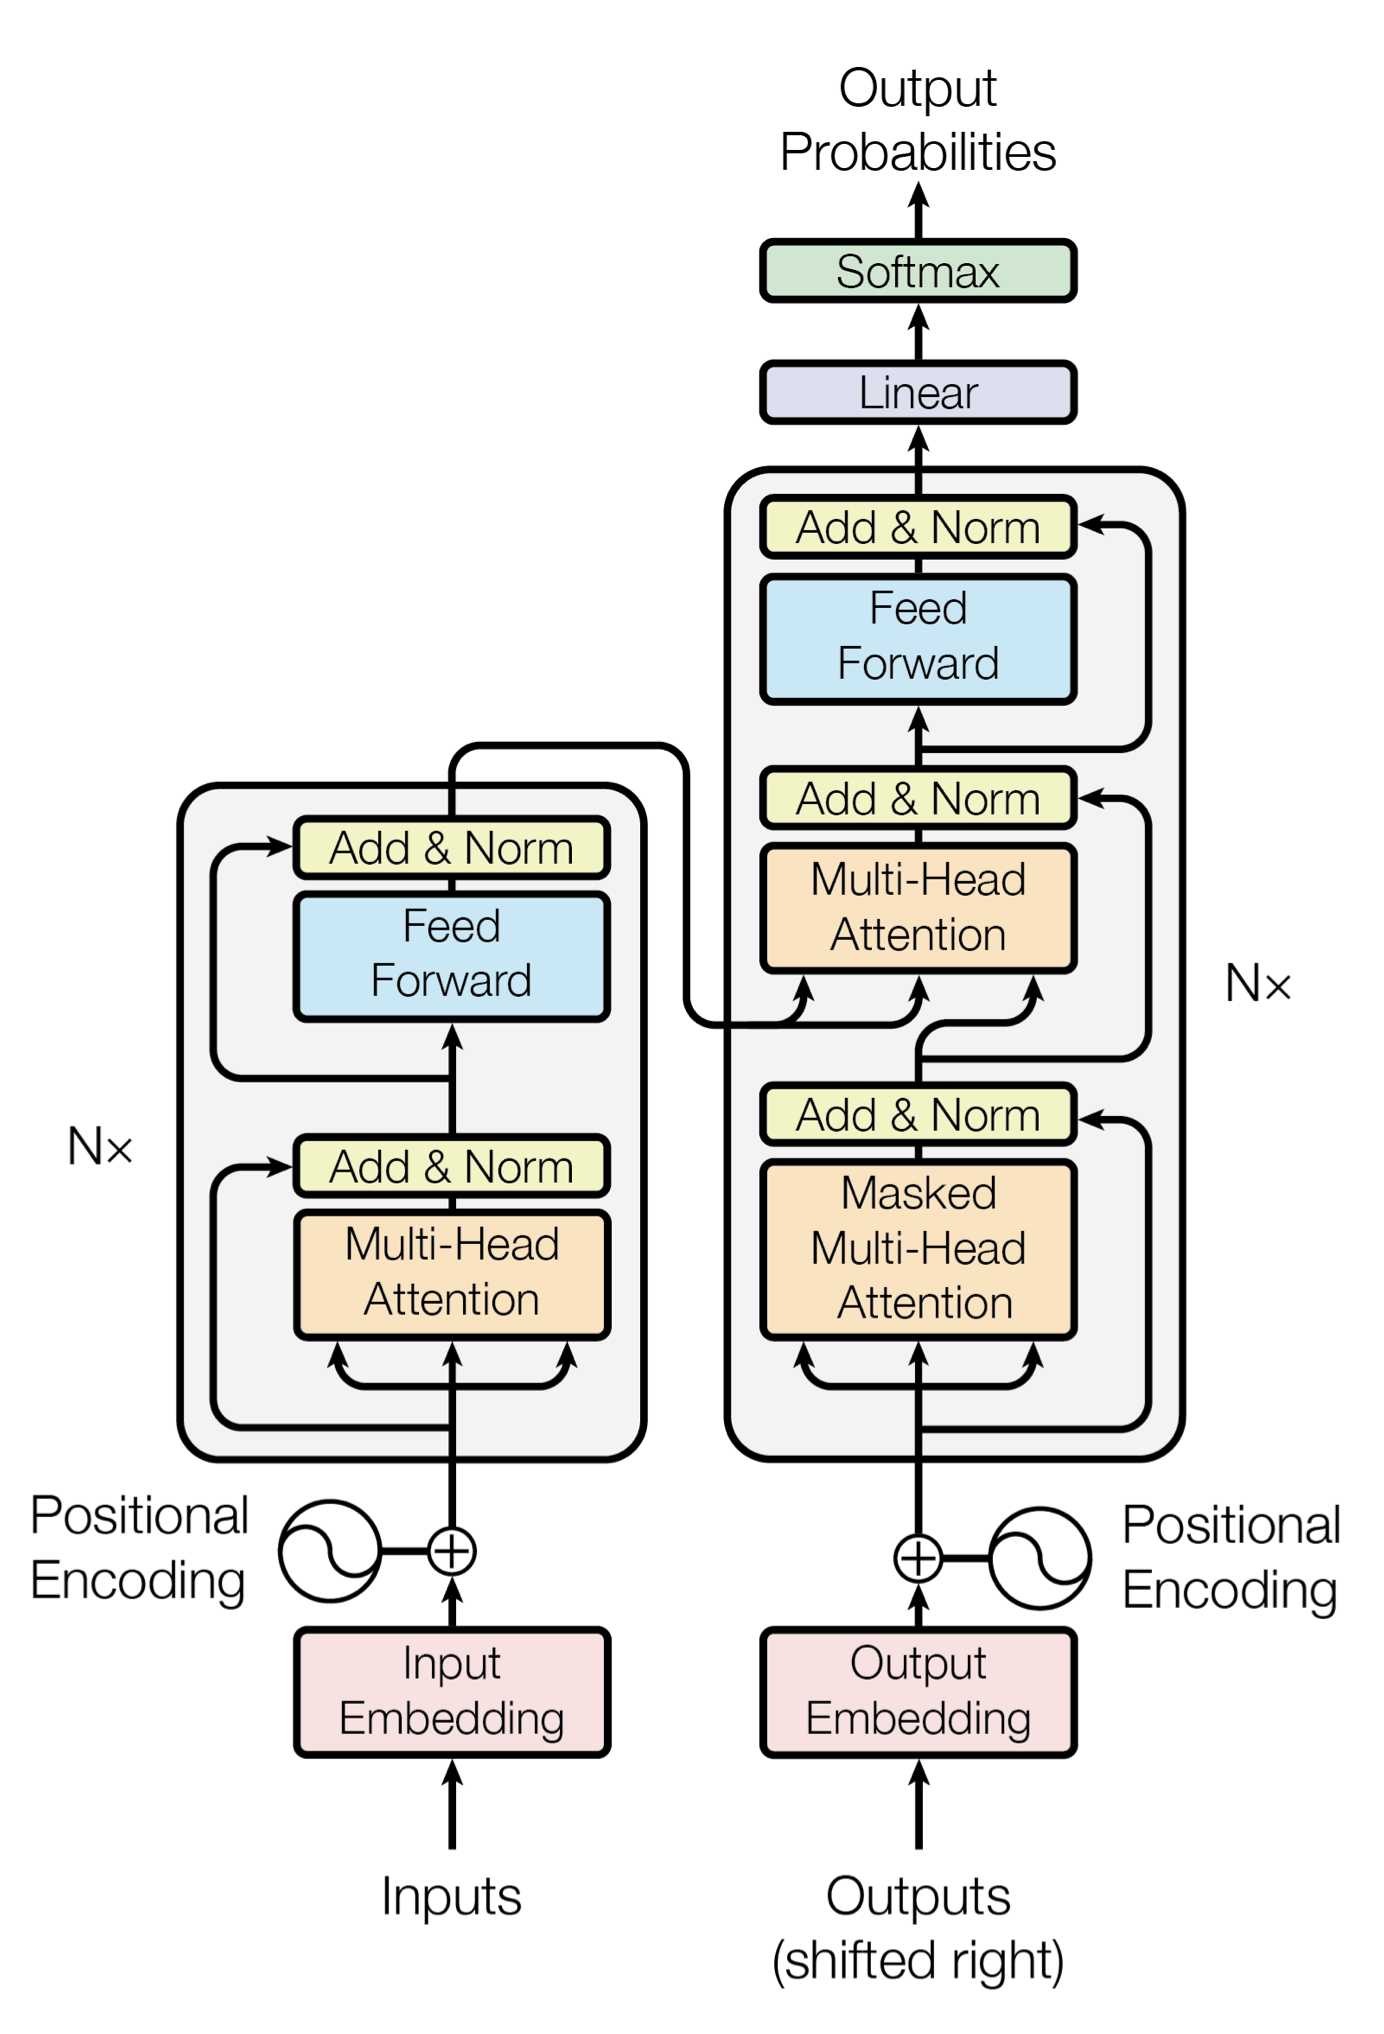
\includegraphics[width=.9\textwidth]{figures/transformer_paper/Transformer_Original.png}
        \caption{Original Transformer Architecture (Image from \textcite{vaswani2017})
        % ]{Traditional transformer architecture consisting of an enocoder and decoder. 
        \label{fig:transformer_orig}}
    \end{figure}
% \end{frame}

% \begin{frame}
\column{.58\textwidth}
    \begin{figure}[t]
        \centering
        \includegraphics[width=\textwidth]{figures/transformer_paper/ViT_Original.png}
        \caption{ViT Architecture (Image from \textcite{dosovitskiy2020})
        % ]{Vision transformer (ViT) architecture. Purple ovals indicate 
        %     positional embeddings, while pink ovals indicate the resulting tokens from 
        %     the patches. 
        \label{fig:ViT_orig}}
    \end{figure}
    \end{columns}
\end{frame}

\begin{comment}
\begin{frame}
    \begin{columns}
        \column{0.4\textwidth}
            This is an example of text and image in the same slide using columns environment.
        \column{0.6\textwidth}
            \begin{figure}
                \centering
                \includegraphics[width=\textwidth]{Neural-Network.jpg}
                \caption{Neural Network with 5 neurons in the hidden layer. }
            \end{figure}
    \end{columns}
\end{frame}

\begin{frame}
    \frametitle{HAM10000 Dataset \cite{Sagar2022}}
        {
            \small
            \begin{table}
            \centering
            \caption{HAM10000 Dataset Classes}\label{tab:HAM}
            \resizebox{.3\linewidth}{!}{\begin{tabular}{lccc}
	\toprule
    \textbf{Spam} & \textbf{Ni} & \textbf{Swallow} & \textbf{Shrubbery} \\
    \midrule
    A & 1 & 2 & 3 \\
    \midrule
    E & 3 & 4 & 5 \\
    C & 6 & 9 & 3 \\
    \midrule
    M & 4 & 1 & 1 \\
    \bottomrule
\end{tabular}}
            \end{table}
        }
        \begin{figure}
            \centering
            
\includegraphics[width=0.3\textwidth]{figures/blackbox.jpeg}
            \caption{Example of HAM10000 dataset with true classes and segmentation}
        \end{figure}
\end{frame}
%%%%%%%%%%%%%%%%%%%%%%%%%%%%%%%%%%%%%%%%%%%%%%%%%%%%%%%%%%%%%%%%%%%%%%%%
\begin{frame}
    \frametitle{Classification Models}
    \small
    \begin{table}[]
        \centering
        \caption{Models}\label{tab:models}
        \resizebox{\linewidth}{!}{\begin{tabular}{lccc}
	\toprule
    \textbf{Spam} & \textbf{Ni} & \textbf{Swallow} & \textbf{Shrubbery} \\
    \midrule
    A & 1 & 2 & 3 \\
    \midrule
    E & 3 & 4 & 5 \\
    C & 6 & 9 & 3 \\
    \midrule
    M & 4 & 1 & 1 \\
    \bottomrule
\end{tabular}}
    \end{table}
    
\end{frame}
\end{comment}